\documentclass[a4paper, 11pt]{article}
\usepackage[utf8]{inputenc}
\usepackage[english]{babel}
\usepackage[breakable]{tcolorbox}
\usepackage{indentfirst}
\usepackage{graphicx}
\usepackage{hyperref}
\usepackage{color} 
\usepackage{multirow}
\usepackage{iftex}
\ifPDFTeX
	\usepackage[T1]{fontenc}
	\usepackage{mathpazo}
\else
	\usepackage{fontspec}
\fi
\usepackage{caption}
% \DeclareCaptionFormat{}{}
% \captionsetup{aboveskip=0pt,belowskip=0pt}

\usepackage{float}
\floatplacement{figure}{H} % forces figures to be placed at the correct location
\usepackage{xcolor} % Allow colors to be defined
\usepackage{enumerate} % Needed for markdown enumerations to work
\usepackage{geometry} % Used to adjust the document margins
\usepackage{amsmath} % Equations
\usepackage{amssymb} % Equations
\usepackage{textcomp} % defines textquotesingle

% Colors for the hyperref package
\definecolor{urlcolor}{rgb}{0,.145,.698}
\definecolor{linkcolor}{rgb}{.71,0.21,0.01}
\definecolor{citecolor}{rgb}{.12,.54,.11}

% Prevent overflowing lines due to hard-to-break entities
\sloppy 
% Setup hyperref package
\hypersetup{
  breaklinks=true,  % so long urls are correctly broken across lines
  colorlinks=true,
  urlcolor=urlcolor,
  linkcolor=linkcolor,
  citecolor=citecolor,
  }
% Slightly bigger margins than the latex defaults

\geometry{verbose,tmargin=1in,bmargin=1in,lmargin=1in,rmargin=1in}
    
    
\begin{document}
    \begin{titlepage}
 \begin{center}
  {\Huge\textsc{Brno University of Technology\\[0.3em]
    \huge{Faculty of Information Technology}}}\\
  \vspace{\stretch{0.352}}
  {\Huge
  Generative image inpainting enhanced with edge focused WGAN-GP adversarial loss.}\\
  \vspace{\stretch{0.06}}
  {\Large Authors: Tomáš Beránek (xberan46), Richard Klem (xklemr00)}
  \vspace{\stretch{0.568}}
 \end{center}
 {\Large 
 \today 
 \hfill
}
\end{titlepage}

\newpage
\section{Abstract}
\label{section:abstract}
We improved the original Yu's \cite{Yu} model by adding a third discriminator. The original solution uses the local discriminator to calculate the loss on the generated patch and the global discriminator to calculate a loss on the whole image. But very often, we can see the edges of the patch, because there is no special attention to smooth transition between the generated patch and the rest of the image. We decided to provide a new discriminator, which will be focusing on the path with the near surroundings. This should help the generator to learn how to make better transitions on the edges of the patch and it should also lead to more clear/sharp patch.

\section{Related work}
\label{section:relatedWork}
According to Jiahui Yu \cite{Yu}, there are two main categories. The first is a diffusion-based or patch-based approach and the second one is a learning-based or attention modeling approach.
The diffusion-based model uses variational algorithms to propagate information from the background regions to the holes. Patch-based approaches use patch similarity to do so. Diffusion and patch-based approaches work well for stationary textures as you can see in figure \ref{img:patchApproach}. The image on the right is generated by joint interpolation of the image gray levels and gradient/isophotes directions. \cite{patch}
On the other side, these methods have decreased the quality of output for non-stationary data such as natural images.
\begin{figure}
    \centering
    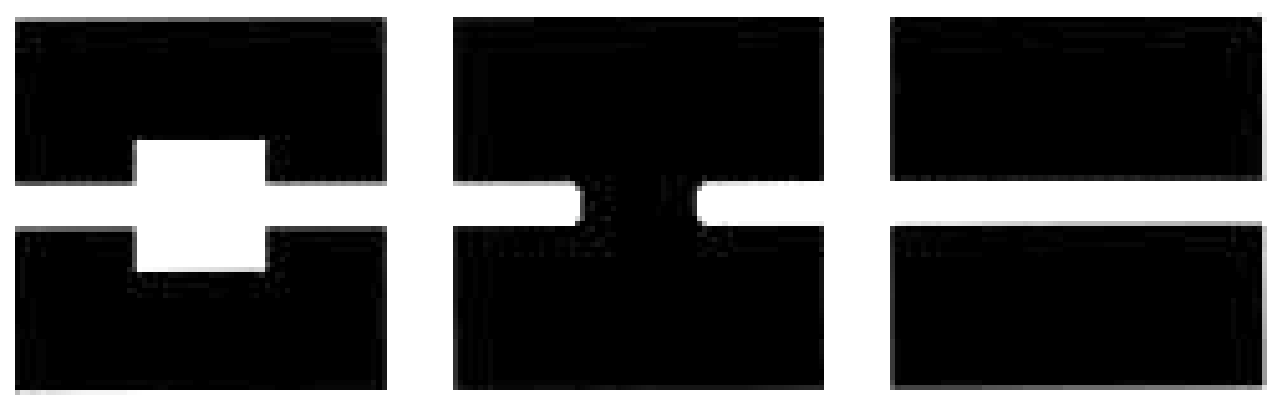
\includegraphics[width=0.95\linewidth]{documentation/img/patchApproach.png}
    \caption{On the left side: the input image with square mask, on the right side: the result from joint interpolation method by Ballester et al.}
    \label{img:patchApproach}
\end{figure}


\section{Dataset}
\label{section:dataset}
This section describes both datasets from the original work and what we used in our work.
Both we, and Yu and al. use Places2 dataset. \footnote{http://places2.csail.mit.edu/} More specifically the high-resolution images, which have been resized to have a minimum dimension of 512 while preserving the aspect ratio of the image. Original images that had a dimension smaller than 512 have been left unchanged.

For time reasons, we decided to use just a subset of the Places2 dataset. We reduced our dataset from the original 365 categories to the 7 categories: \textit{army\_base}, \textit{badlands}, \textit{corn\_field},
\textit{forest\_path}, \textit{golf\_course}, \textit{hayfield} and \textit{mountain}. 
Each category has always 5000 images. We split it in a certain ratio, so we have a training dataset containing 4500 images and a testing dataset containing 500 images from each category.
It makes 35 thousand pictures in total. 31 500 images serve as a training set. 3500 pictures were selected as testing/validation set.

\section{The original work and article}
\label{section:origin}
The Yu's \cite{Yu} solution is based on the work of \cite{Iizuka} named \textit{Globally and
locally consistent image completion}. Yu et al. improved this approach with various changes and additions. 
In figure \ref{img:iizukaArch} you can see the architecture of the Iizuka et al. model. It is worth mentioning for future reference that the completion network is one piece network and that the outputs of local and global discriminators are merged.

The one of the main changes is split of completion network into two stages -- coarse-to-fine network. Coarse network (the first stage) makes an initial coarse prediction. Then the refinement network (the second stage) takes the coarse prediction as input and predict refined result. With this split is connected also the way of using values of loss functions.
The coarse network is trained with the reconstruction loss explicitly, while the refinement network is trained with the reconstruction loss as well as GAN losses. They also removed the batch normalization layers, which they found deteriorates color coherence.

In the Iizuka's \cite{Iizuka} work is used concatenation layer, which concatenates outputs from local and global discriminator. But Yu et al. found, that it is better if they keep the outputs from discriminators separate. Regarding GAN architecture, in the Yu's work, they used Wasserstein GANs as opposed to DSGANs used in Iizuka's work. More specifically, Yu et al. used WGAN-GP. They also stated. that WGAN-GP losse works well when combined with $\ell_1$
reconstruction loss as they both use the $\ell_1$ distance metric.

To prevent pixel hallucination and very different content in the center of the generated patch, Yu et al. introduce spatially discounted reconstruction loss using a weight mask. 
The weight of each pixel in the mask is computed as $\gamma^l$, where $l$ is the distance of the pixel to the nearest known (not masked) pixel. $\gamma$ is set to 0.99 in all experiments. They use
discounted $\ell_1$ reconstruction loss in their implementation.

All these changes and improvements made by Yu et al. leads to faster convergence (as far as we can speak about convergence in generative models) than the Iizuku's work. Also it resulted in more accurate inpainting outputs. Yu stated a 100x speedup, nevertheless we personally take it with a grain of salt as the proposed numbers does not correspond well with whe Iizuka's paper.

\begin{figure}
    \centering
    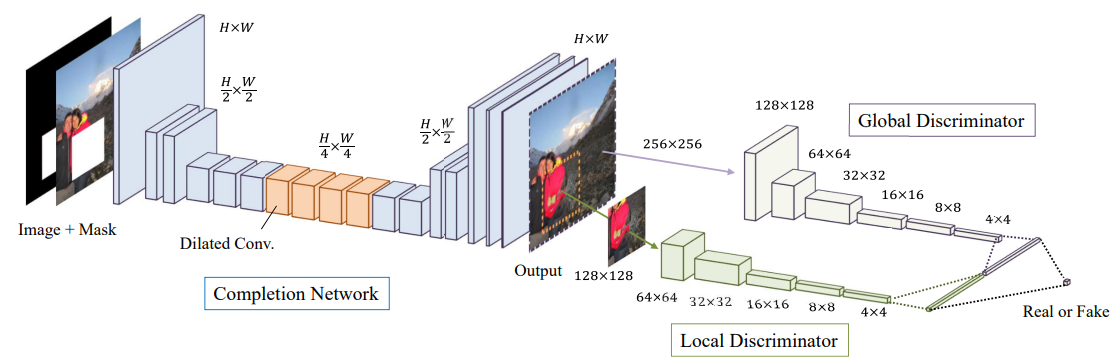
\includegraphics[width=0.95\linewidth]{documentation/img/iizukaArch.png}
    \caption{Architecture proposed by Iizuka et al. based on one completion generative network and two discriminators.}
    \label{img:iizukaArch}
\end{figure}


\begin{figure}
    \centering
    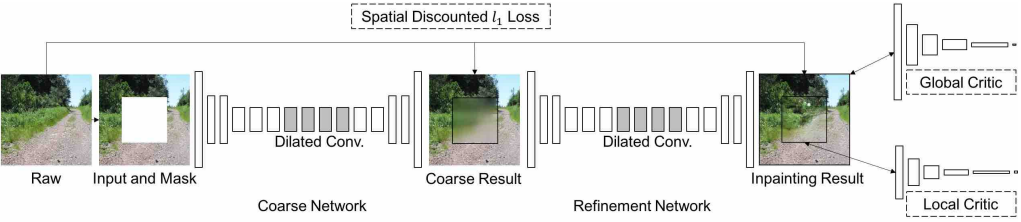
\includegraphics[width=0.95\linewidth]{documentation/img/original_arch.png}
    \caption{Architecture modified by Yu et al. You can see generative network split to coarse and refinement network and discriminators kept separated.}
    \label{img:yuArch}
\end{figure}


\section{Our enhanced solution -- edge focused discriminator}
\label{section:edgeDiscriminator}
We have noticed that Yu's \cite{Yu} results are high quality, but there is often observable transition between the generated patch and the rest of the image. We were thinking about how to improve this aspect and we thought we could add another discriminator, which will be focused on the edges of the patch and the near surrounding. We want to smooth the transition between the patch and the rest of the image and more sharp patch itself. For these purposes we used the Sobel edge detector.

To detect edges in the patch we choose to use Sobel edge detection\footnote{\href{https://www.tensorflow.org/api_docs/python/tf/image/sobel_edges?authuser=1}{https://www.tensorflow.org/api\_docs/python/tf/image/sobel\_edges?authuser=1}}. This method is able to detect both vertical and horizontal edges in the image. It is detecting all edges in the input image, so we had to create special input for this method to successfully use it for our use-case.
First we convert image to the gray-scale and then the Sobel edge detection is applied.
The ouput of the Sobel edge detector is an image with the same dimensions but each pixel is converted to the white when it is considered as an edge or black if it is not. How the Sobel edge detection works can be seen in figure \ref{img:sobel} which has been taken from Verma et al. work \cite{sobel}.
\begin{figure}
    \centering
    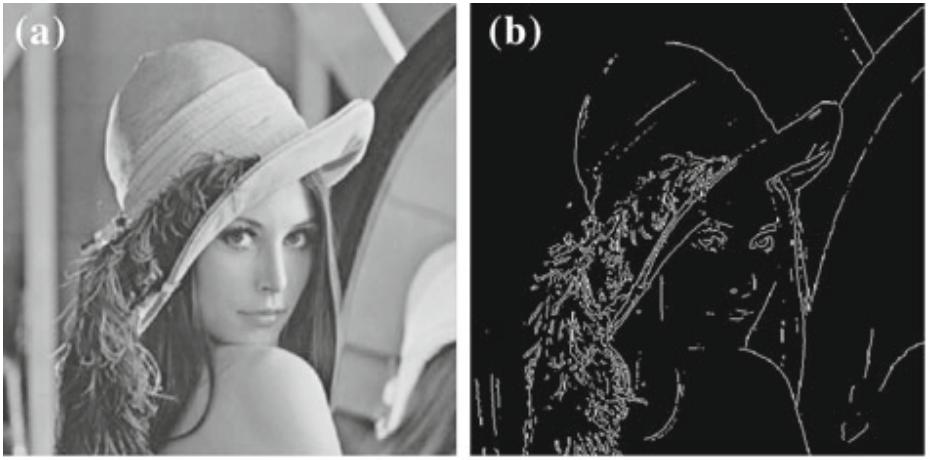
\includegraphics[width=0.65\linewidth]{documentation/img/sobel.png}
    \caption{a) The original image converted to the gray-scale, b) Output from Sobel edge detection.\cite{sobel}}
    \label{img:sobel}
\end{figure}

The Sobel edge detection is part of the edges discriminator. Similarly to the other two discriminators, the output of the Sobel edge detection is followed by a few convolution layers, which results to binary classification -- \textit{real or fake}. The Sobel edge detection can be understood as some pre-processing.

For the ability to a proper comparison of Yu's model with our improved model, we decided to train the model with the same settings as Yu et al. That is why we use a random selection of the input image cropped to 256x256 pixels. For example, if the input image has a size of 734x512 pixels, the algorithm randomly selects an area of 256x256 pixels. In that cropped input image, there is randomly cut off the mask of the size of 128x128 pixels.
While creating the input data (referenced as \textit{edges patch} furthermore) for the edges discriminator, we took the local patch but with an extra 16 pixels added in each direction. The final size of this edges patch is therefore +32 pixels in both height and width. For our particular case, it means 160x160 pixels (128+32=160).
You can see our improved architecture in figure \ref{img:ourArch}
\begin{figure}
    \centering
    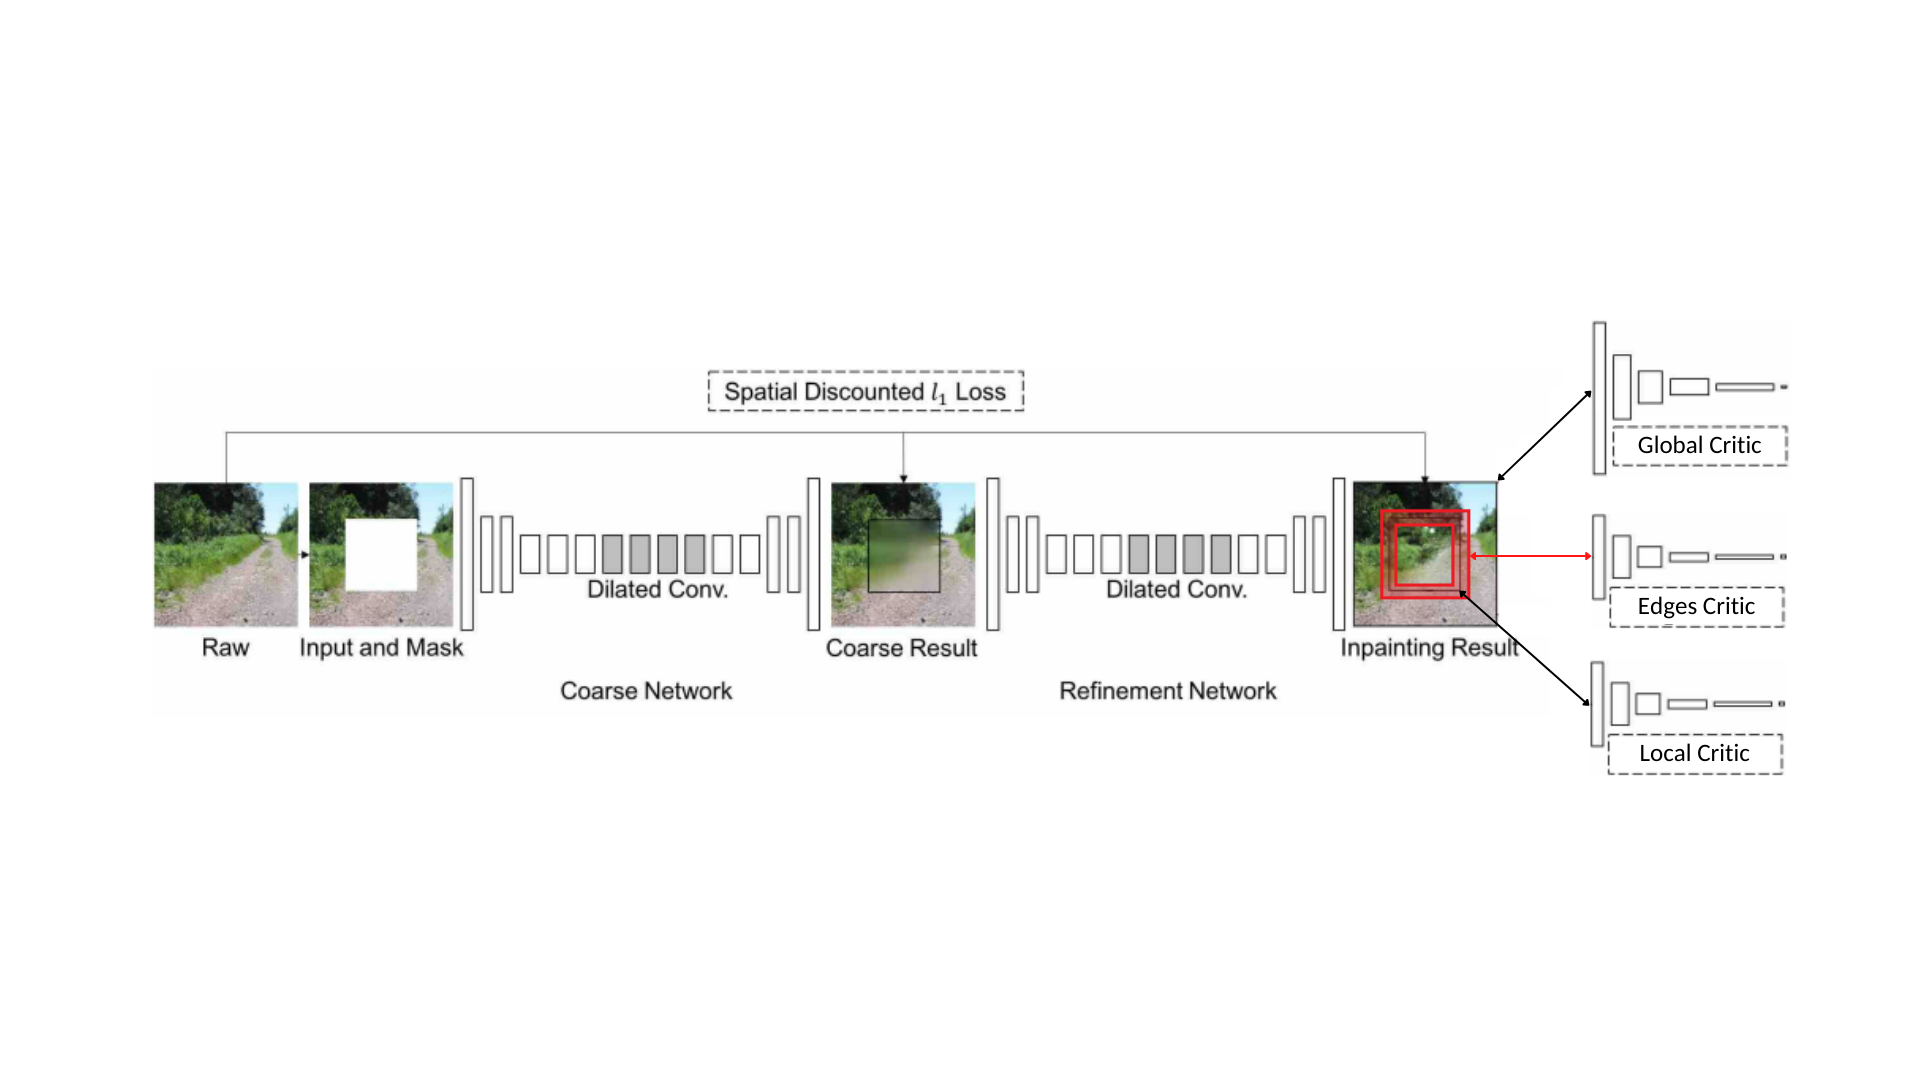
\includegraphics[width=0.95\linewidth]{documentation/img/new_arch.png}
    \caption{Our improved architecture with extra discriminator focus on edges of the generated patch and the near surrounding.}
    \label{img:ourArch}
\end{figure}

Yu's solution uses a simple sum of losses from the global and local discriminator. We followed the same approach and we have added loss from edges discriminator to the previous ones. Regards the weights they are the same, set to $\alpha = 1.0$. So the formula for the overall loss from all three WGAN-GP discriminators is $losses=1.0*loss_{global} + 1.0*loss_{local} + 1.0*loss_{edges}$.

The rest of the logic of the model remained untouched. That means we did not change any part of the generator nor any of the original discriminators. We have enhanced what was already working well.

\section{Training, testing and validation}
\label{section:training}
We have trained both the baseline and our modified model from scratch, so we can do a meaningful comparison.
Because we were training on our machines, we had to modify the original batch size from 16 to 8 images.
We trained both the original and our model for 100,000 iterations. We set the training process to save checkpoint models during the training process, so we can do a comparison if the generator is improving along with the training.
As already discussed in section \ref{section:dataset} we have trained on seven categories, with 4500 images each category.

The validation and testing of generative models are very tricky and difficult.
There are many methods to evaluate the technical properties of an image, but it is difficult to use them to validate that generator is generating some meaningful human-eye pleasant output. 
The generator could produce nonsense, but with nice SNR, and then it will be evaluated as a good quality image.

The most accurate measurement of the image looks nice and natural is manual testing. We were able to manage several manual testing sessions. The task of this manual testing was choosing between two images, which one did the users like more. If the users were not sure where are the differences, the users could show the mask so they can focus on that/these specific parts of the images.
Overall we collected 629 comparisons from 6 unique people and 177 unique images.
The results are the following:
\begin{itemize}
    \item 67.23\% (119/177) of images from our model were voted as better compared to the 32.77\% (58/177) from Yu's model.
    \item 66.61\% (419/629) of votes were for our model compared to the 33.39\% (210/629) for Yu's model.
\end{itemize}

\section{Experiments}
\label{section:experiments}
We did some experiments with activation functions in the generator. We tried to use Swish instead of ELU according to the blog article of Andre Ye\cite{Ye_swish}. The Swish activation function should be the very best alternative to ReLU, but according to the experiments proposed in the article, Swish should also outperform ELU in eight of nine cases. But unfortunately for us, we cannot confirm this in our particular use case. The output of the generator was not better, because it creates a style of \textit{"oil in the water puddle"}, which was not desired.
You can see the swish properties in the figure \ref{img:swish}.

\begin{figure}
    \centering
    \begin{minipage}{.48\textwidth}
      \centering
      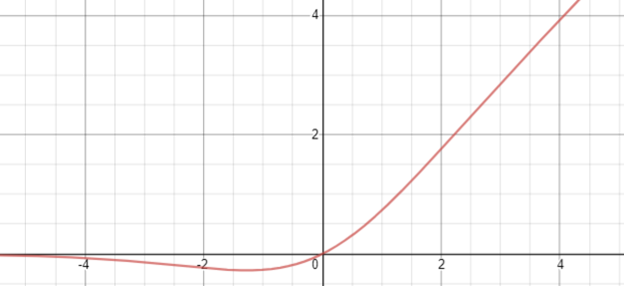
\includegraphics[width=.95\linewidth]{documentation/img/swish.png}
    \end{minipage}%
    \begin{minipage}{.49\textwidth}
      \centering
      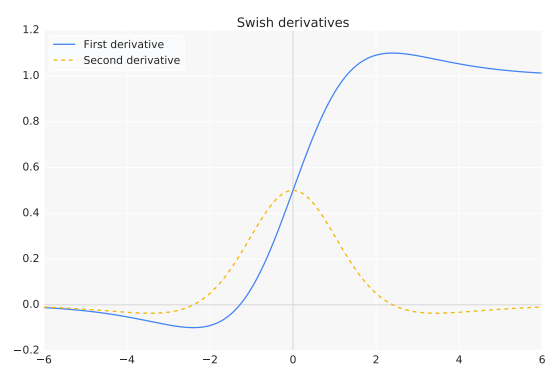
\includegraphics[width=.95\linewidth]{documentation/img/swish_derivates.png}
    \end{minipage}
    \caption{Swish activation function properties. Taken from Ye's work.\cite{Ye_swish}}
    \label{img:swish}
\end{figure}

For furthermore development, there is plenty of space. Some other, maybe more advanced/accurate methods of edge detection could be used. In the original Yu's solution there is used ReLU at one place, which is the end of convolution layers series in contextual attention. We expect, that in this specific case the ReLU could be replaced with the swish function with success.
Another experiment can be done by normalizing discriminators' loss sum. The original solution uses the same $\alpha=1$ and we kept to this. But it could be interesting to experiment with $\alpha=\frac{2}{3}$ or so.

\section{Results and conclusions}
\label{section:results}
We came up with an improvement of the state-of-the-art approach. We managed to implement this enhancement successfully.
We have done some experiments and stated what are other possibilities on how to improve this model.
Also, we have done extensive manual testing with multiple users and plenty of example images for both models and we evaluated that our improved model generates about twice as many human-eye pleasant images as the original one.
According to the manual testing results, image sharpness analysis, and based on provided examples below, we can state, that we have enhanced the smoothness of the transition between the edges of the patch and the rest of the image.
There are some examples in which it can be seen the difference between the original and our model.
For each example there is at first the mask, the second is the output of Yu's model, and then third, the last one is our output.
\begin{figure}
    \centering
    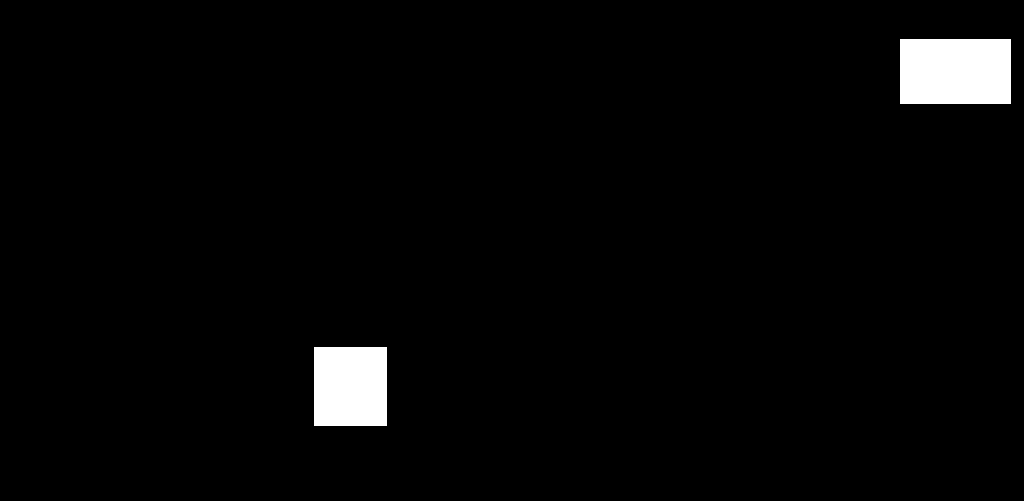
\includegraphics[width=.95\linewidth]{documentation/img/masks/0001_mask.png}
    \caption{Example n.1 -- mask.}
    \label{img:ex_n.1_mask}
\end{figure}
\begin{figure}
    \centering
    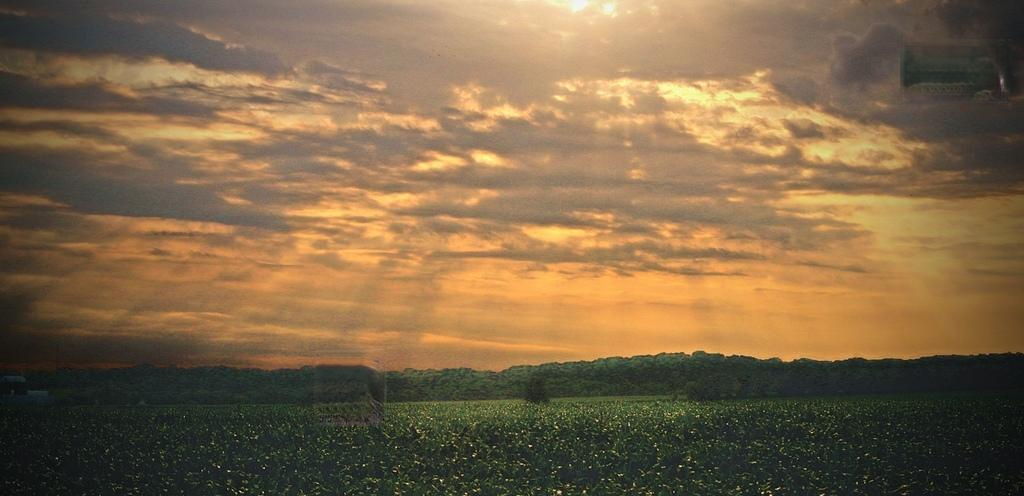
\includegraphics[width=.95\linewidth]{documentation/img/baseline/0001.png}
    \caption{Example n.1 -- Yu (baseline).}
    \label{img:ex_n.1_mask}
\end{figure}
\begin{figure}
    \centering
    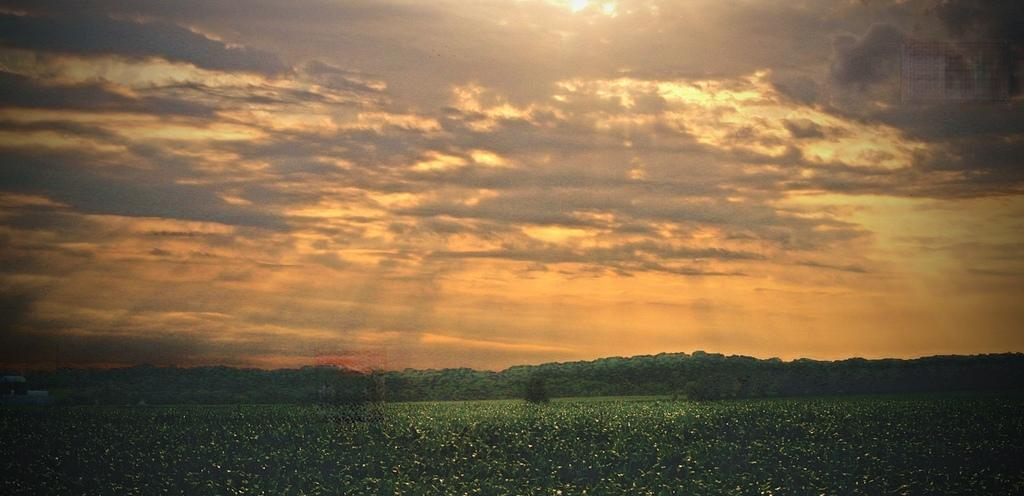
\includegraphics[width=.95\linewidth]{documentation/img/modified/0001.png}
    \caption{Example n.1 -- ours.}
    \label{img:ex_n.1_mask}
\end{figure}

\begin{figure}
    \centering
    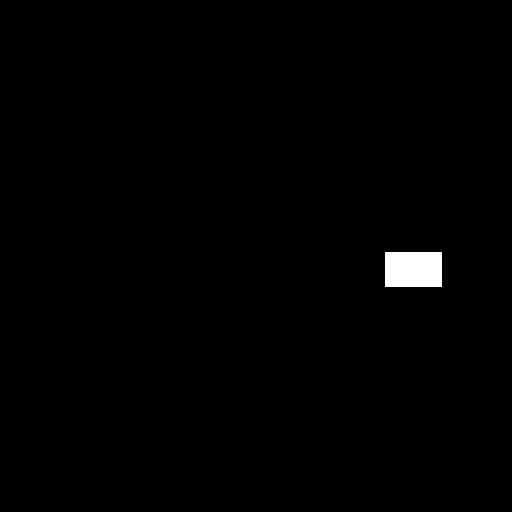
\includegraphics[width=.95\linewidth]{documentation/img/masks/0008_mask.png}
    \caption{Example n.2 -- mask.}
    \label{img:ex_n.2_mask}
\end{figure}
\begin{figure}
    \centering
    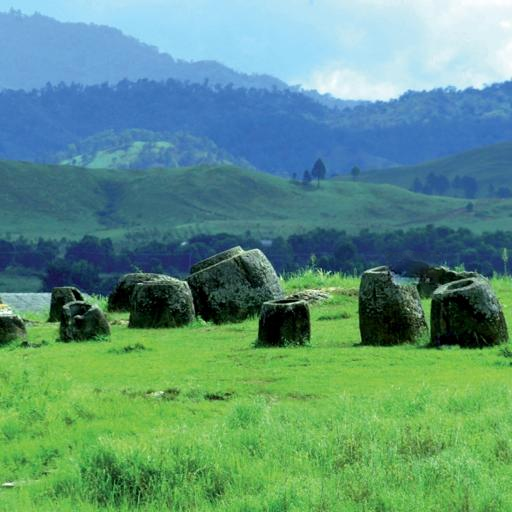
\includegraphics[width=.95\linewidth]{documentation/img/baseline/0008.png}
    \caption{Example n.2 -- Yu (baseline).}
    \label{img:ex_n.2_mask}
\end{figure}
\begin{figure}
    \centering
    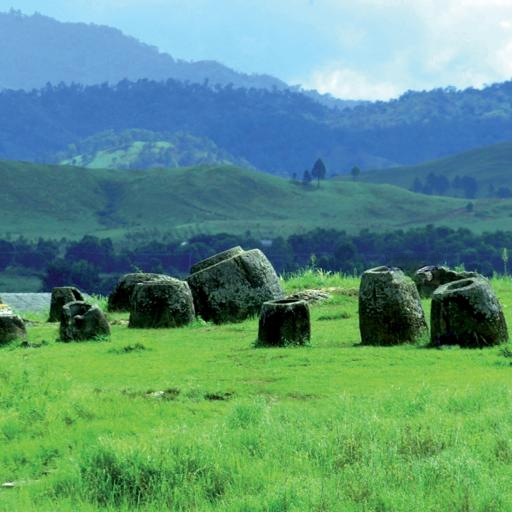
\includegraphics[width=.95\linewidth]{documentation/img/modified/0008.png}
    \caption{Example n.2 -- ours.}
    \label{img:ex_n.2_mask}
\end{figure}

\begin{figure}
    \centering
    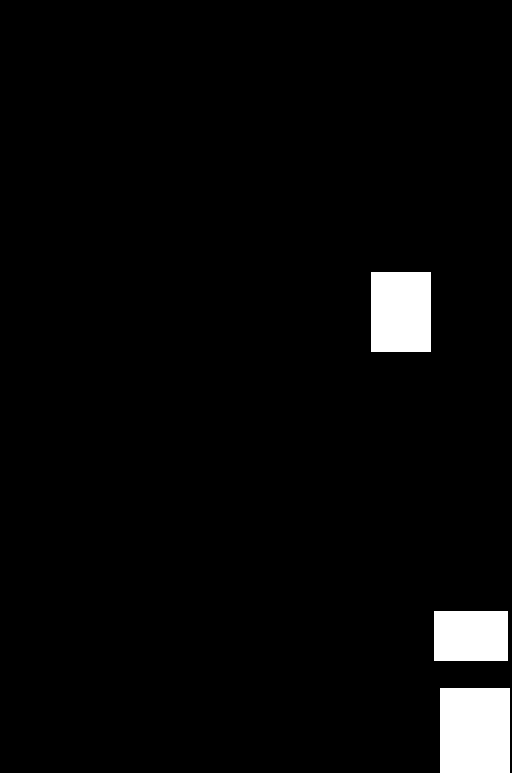
\includegraphics[width=.95\linewidth]{documentation/img/masks/0027_mask.png}
    \caption{Example n.3 -- mask.}
    \label{img:ex_n.3_mask}
\end{figure}
\begin{figure}
    \centering
    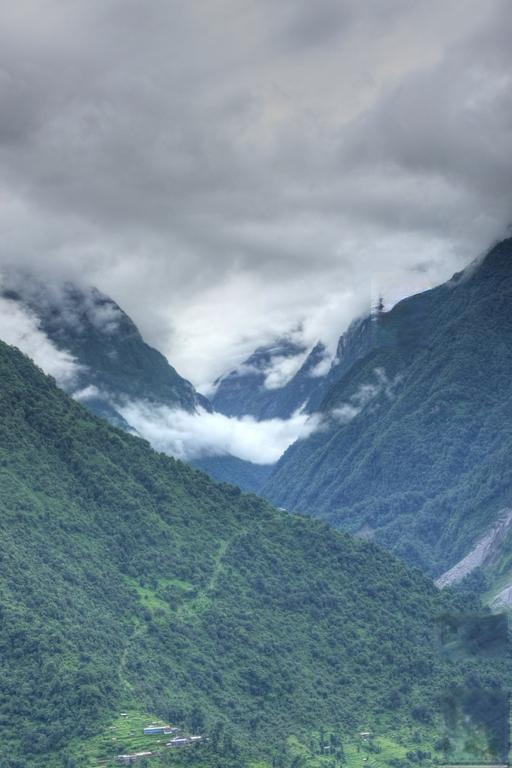
\includegraphics[width=.95\linewidth]{documentation/img/baseline/0027.png}
    \caption{Example n.3 -- Yu (baseline).}
    \label{img:ex_n.3_mask}
\end{figure}
\begin{figure}
    \centering
    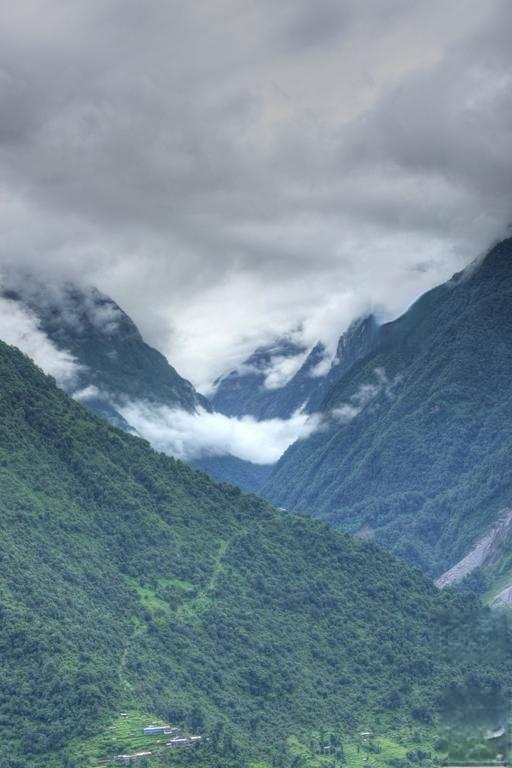
\includegraphics[width=.95\linewidth]{documentation/img/modified/0027.png}
    \caption{Example n.3 -- ours.}
    \label{img:ex_n.3_mask}
\end{figure}

\begin{figure}
    \centering
    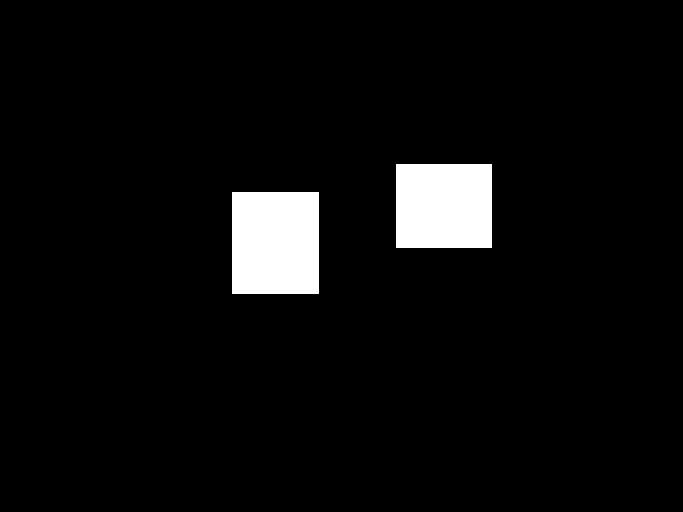
\includegraphics[width=.95\linewidth]{documentation/img/masks/0031_mask.png}
    \caption{Example n.4 -- mask.}
    \label{img:ex_n.4_mask}
\end{figure}
\begin{figure}
    \centering
    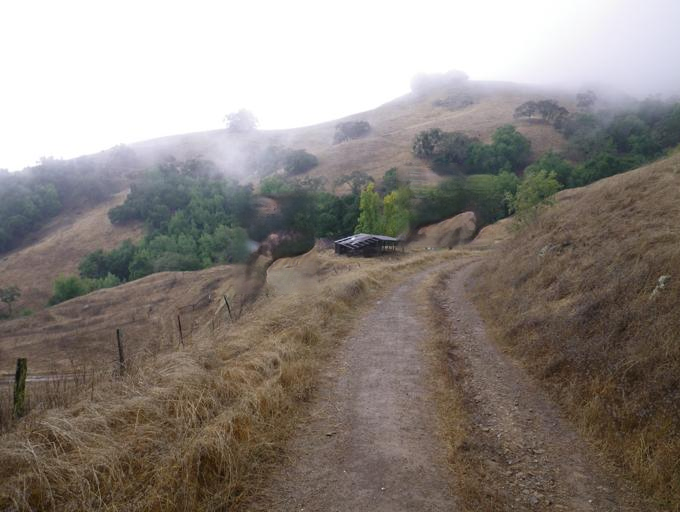
\includegraphics[width=.95\linewidth]{documentation/img/baseline/0031.png}
    \caption{Example n.4 -- Yu (baseline).}
    \label{img:ex_n.4_mask}
\end{figure}
\begin{figure}
    \centering
    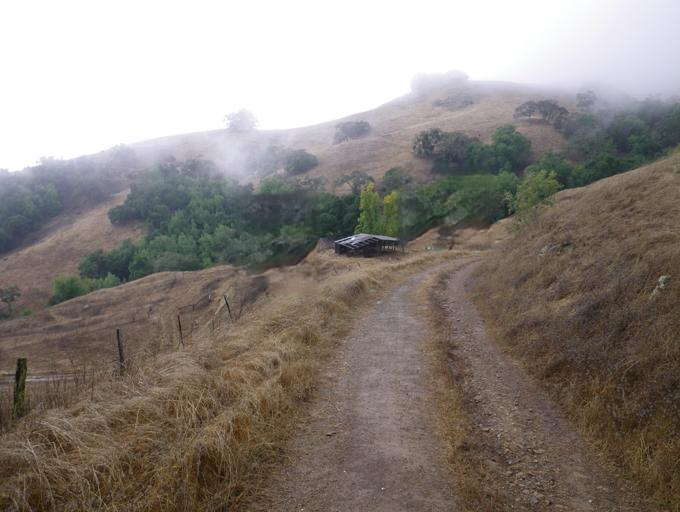
\includegraphics[width=.95\linewidth]{documentation/img/modified/0031.png}
    \caption{Example n.4 -- ours.}
    \label{img:ex_n.4_mask}
\end{figure}

\begin{figure}
    \centering
    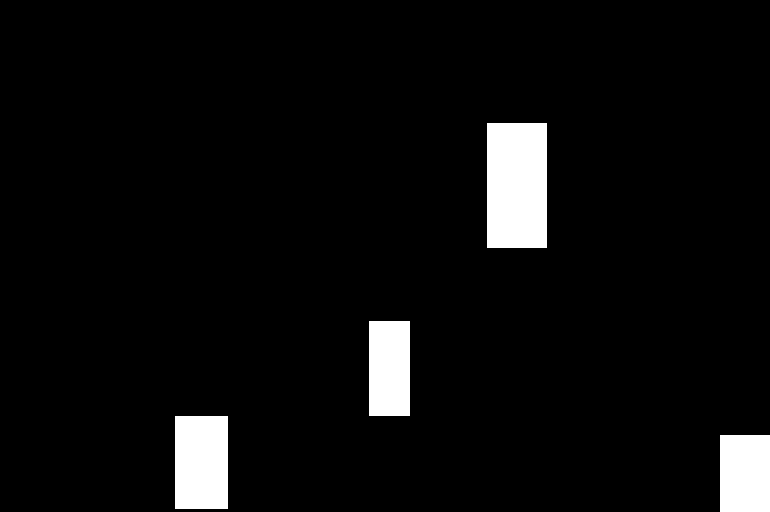
\includegraphics[width=.95\linewidth]{documentation/img/masks/0032_mask.png}
    \caption{Example n.5 -- mask.}
    \label{img:ex_n.5_mask}
\end{figure}
\begin{figure}
    \centering
    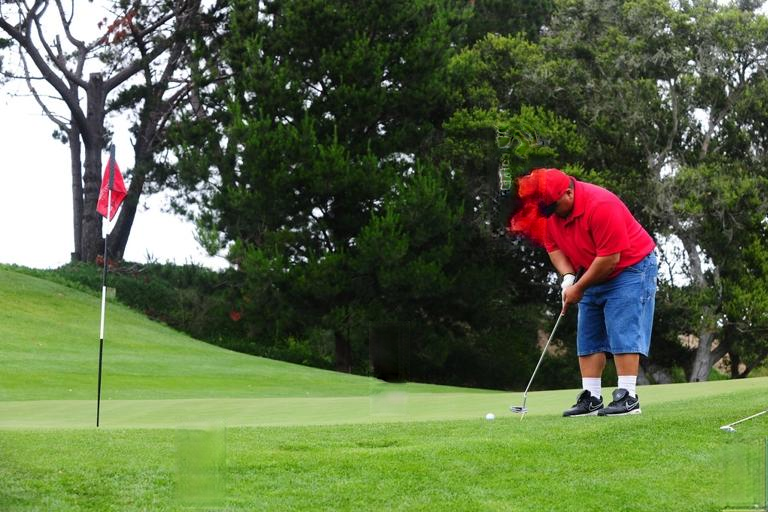
\includegraphics[width=.95\linewidth]{documentation/img/baseline/0032.png}
    \caption{Example n.5 -- Yu (baseline).}
    \label{img:ex_n.5_mask}
\end{figure}
\begin{figure}
    \centering
    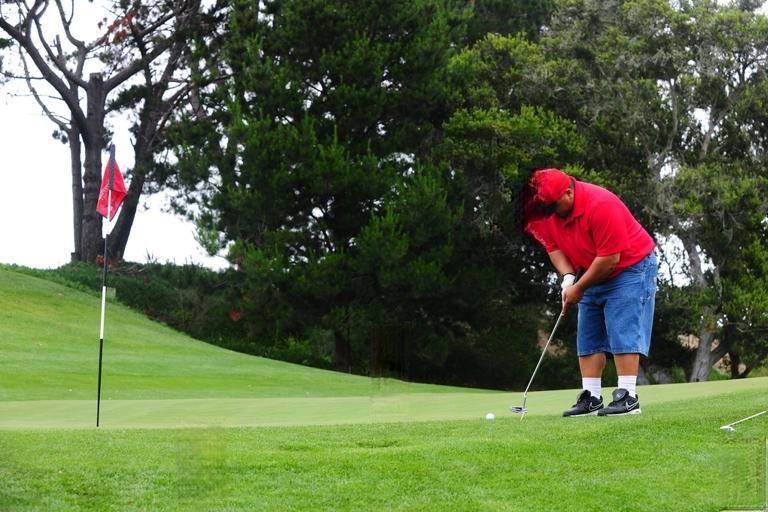
\includegraphics[width=.95\linewidth]{documentation/img/modified/0032.png}
    \caption{Example n.5 -- ours.}
    \label{img:ex_n.5_mask}
\end{figure}

\begin{figure}
    \centering
    
\includegraphics[width=.95\linewidth]{documentation/img/masks/0041_mask.png}
    \caption{Example n.6 -- mask.}
    \label{img:ex_n.6_mask}
\end{figure}
\begin{figure}
    \centering
    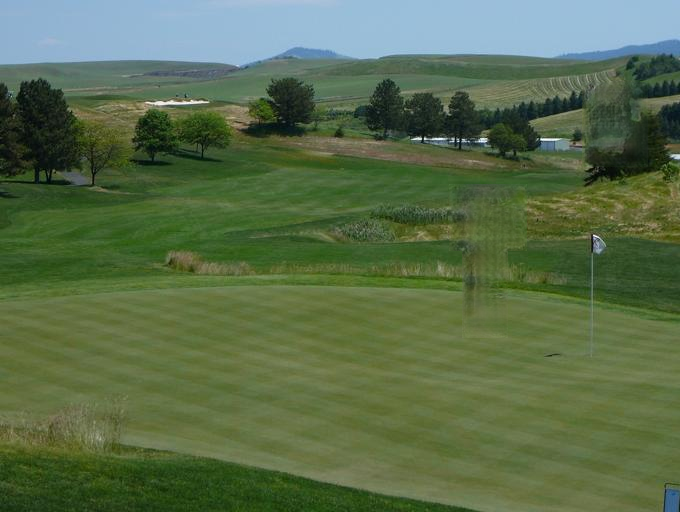
\includegraphics[width=.95\linewidth]{documentation/img/baseline/0041.png}
    \caption{Example n.6 -- Yu (baseline).}
    \label{img:ex_n.6_mask}
\end{figure}
\begin{figure}
    \centering
    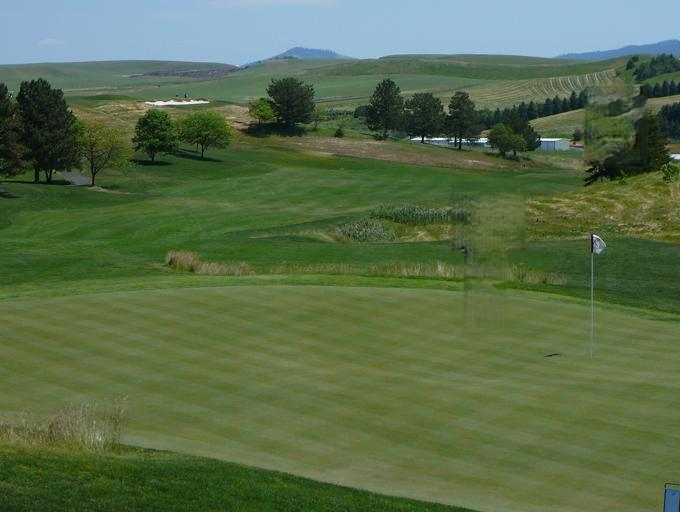
\includegraphics[width=.95\linewidth]{documentation/img/modified/0041.png}
    \caption{Example n.6 -- ours.}
    \label{img:ex_n.6_mask}
\end{figure}

\begin{figure}
    \centering
    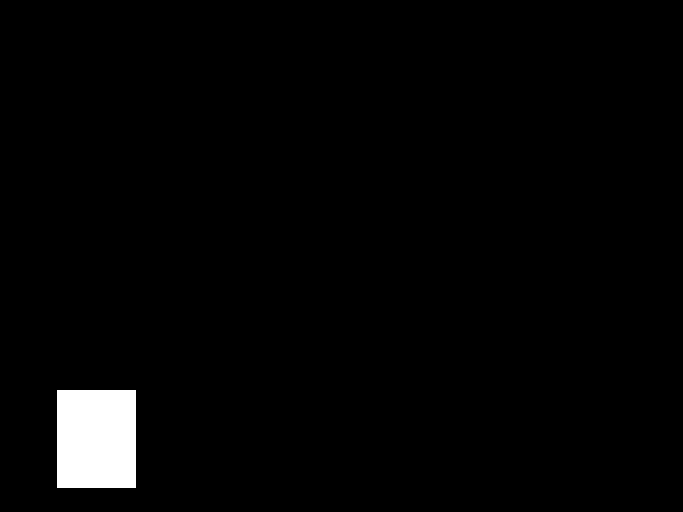
\includegraphics[width=.95\linewidth]{documentation/img/masks/0064_mask.png}
    \caption{Example n.7 -- mask.}
    \label{img:ex_n.7_mask}
\end{figure}
\begin{figure}
    \centering
    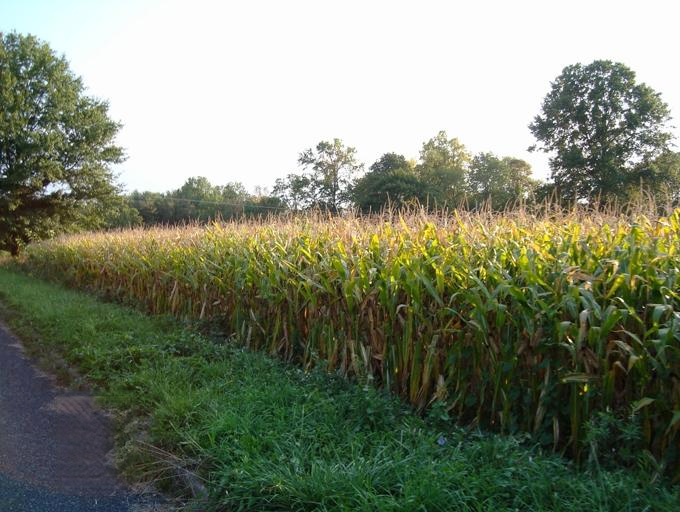
\includegraphics[width=.95\linewidth]{documentation/img/baseline/0064.png}
    \caption{Example n.7 -- Yu (baseline).}
    \label{img:ex_n.7_mask}
\end{figure}
\begin{figure}
    \centering
    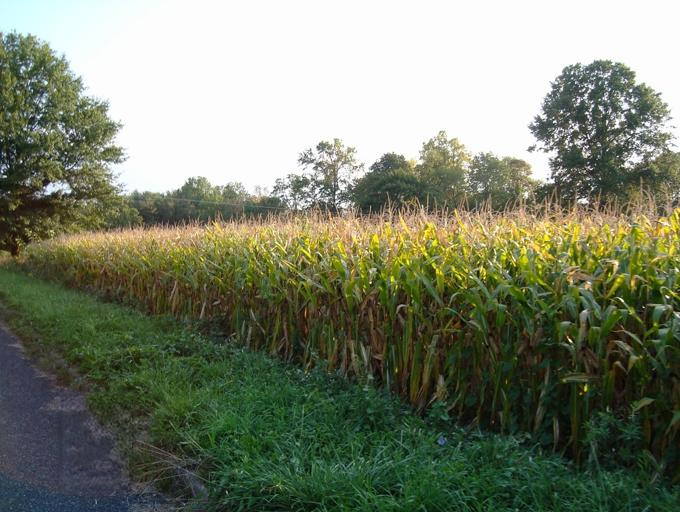
\includegraphics[width=.95\linewidth]{documentation/img/modified/0064.png}
    \caption{Example n.7 -- ours.}
    \label{img:ex_n.7_mask}
\end{figure}

\begin{figure}
    \centering
    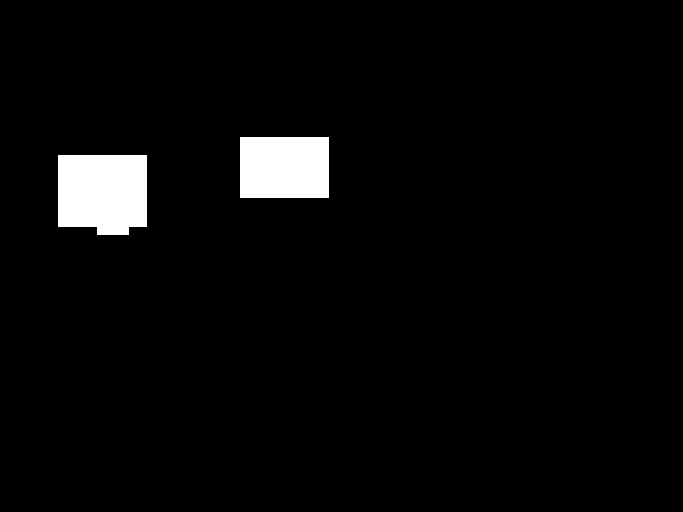
\includegraphics[width=.95\linewidth]{documentation/img/masks/0084_mask.png}
    \caption{Example n.8 -- mask.}
    \label{img:ex_n.8_mask}
\end{figure}
\begin{figure}
    \centering
    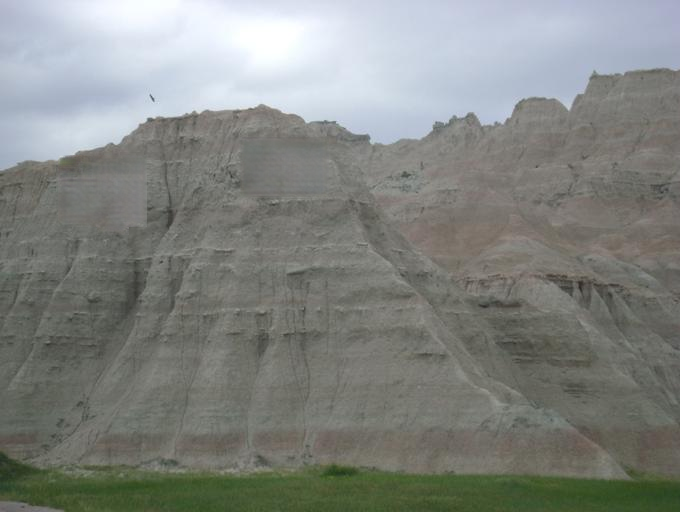
\includegraphics[width=.95\linewidth]{documentation/img/baseline/0084.png}
    \caption{Example n.8 -- Yu (baseline).}
    \label{img:ex_n.8_mask}
\end{figure}
\begin{figure}
    \centering
    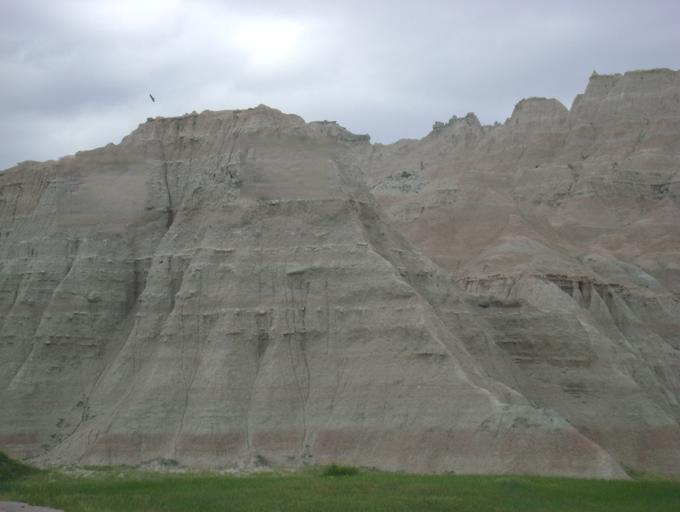
\includegraphics[width=.95\linewidth]{documentation/img/modified/0084.png}
    \caption{Example n.8 -- ours.}
    \label{img:ex_n.8_mask}
\end{figure}

\begin{figure}
    \centering
    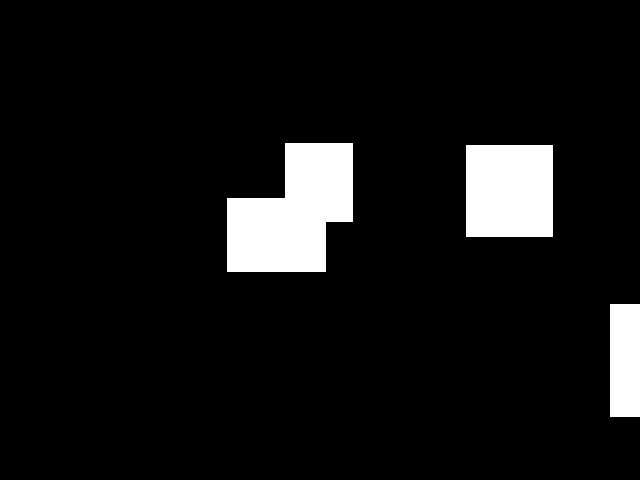
\includegraphics[width=.95\linewidth]{documentation/img/masks/0090_mask.png}
    \caption{Example n.9 -- mask.}
    \label{img:ex_n.9_mask}
\end{figure}
\begin{figure}
    \centering
    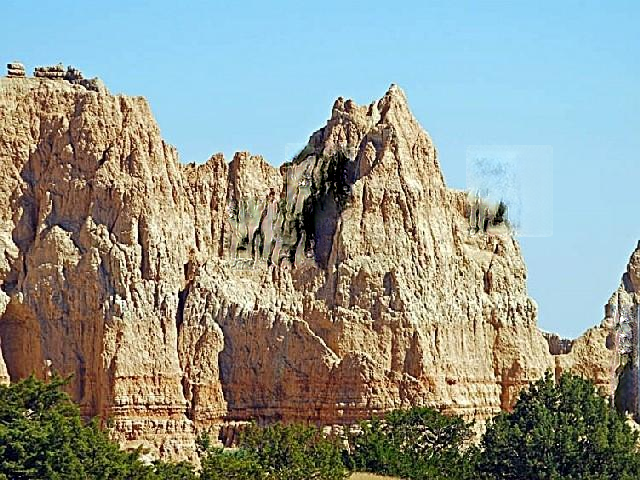
\includegraphics[width=.95\linewidth]{documentation/img/baseline/0090.png}
    \caption{Example n.9 -- Yu (baseline).}
    \label{img:ex_n.9_mask}
\end{figure}
\begin{figure}
    \centering
    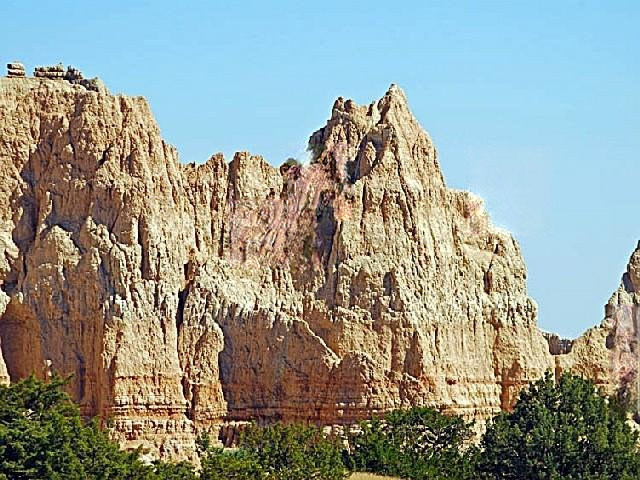
\includegraphics[width=.95\linewidth]{documentation/img/modified/0090.png}
    \caption{Example n.9 -- ours.}
    \label{img:ex_n.9_mask}
\end{figure}


\begin{figure}
    \centering
    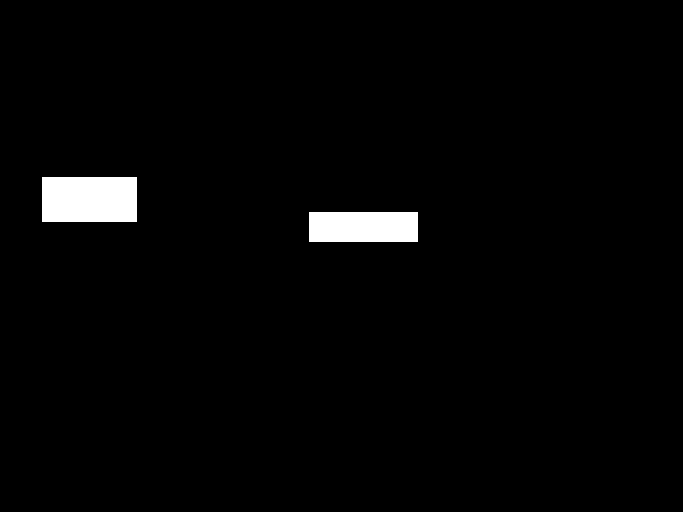
\includegraphics[width=.95\linewidth]{documentation/img/masks/0114_mask.png}
    \caption{Example n.10 -- mask.}
    \label{img:ex_n.10_mask}
\end{figure}
\begin{figure}
    \centering
    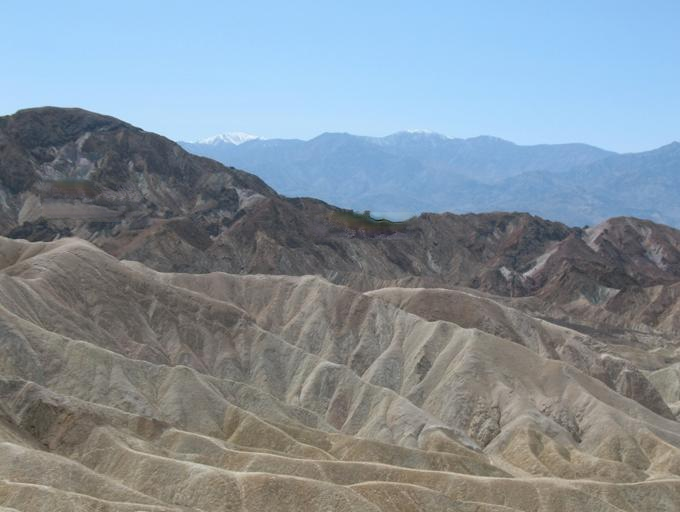
\includegraphics[width=.95\linewidth]{documentation/img/baseline/0114.png}
    \caption{Example n.10 -- Yu (baseline).}
    \label{img:ex_n.10_mask}
\end{figure}
\begin{figure}
    \centering
    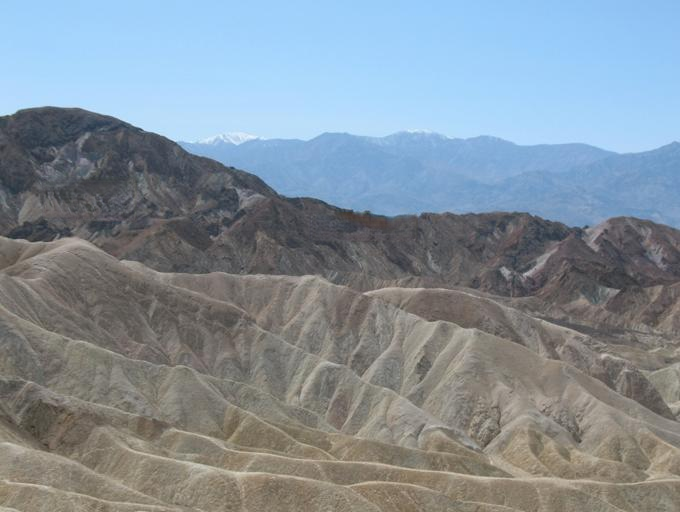
\includegraphics[width=.95\linewidth]{documentation/img/modified/0114.png}
    \caption{Example n.10 -- ours.}
    \label{img:ex_n.10_mask}
\end{figure}

\begin{figure}
    \centering
    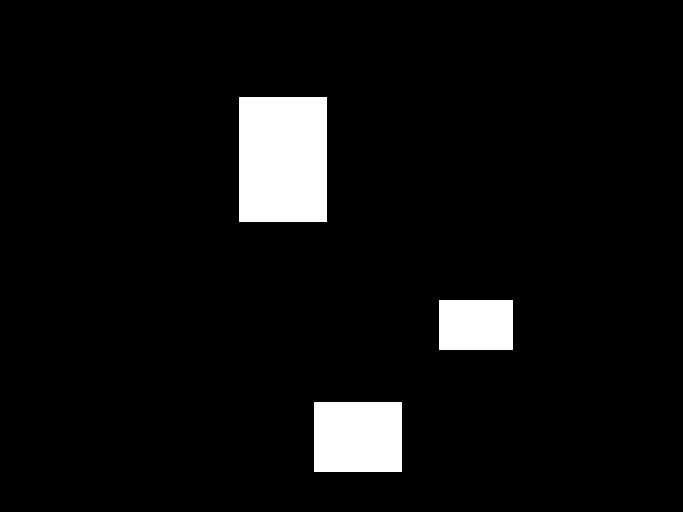
\includegraphics[width=.95\linewidth]{documentation/img/masks/0185_mask.png}
    \caption{Example n.11 -- mask.}
    \label{img:ex_n.11_mask}
\end{figure}
\begin{figure}
    \centering
    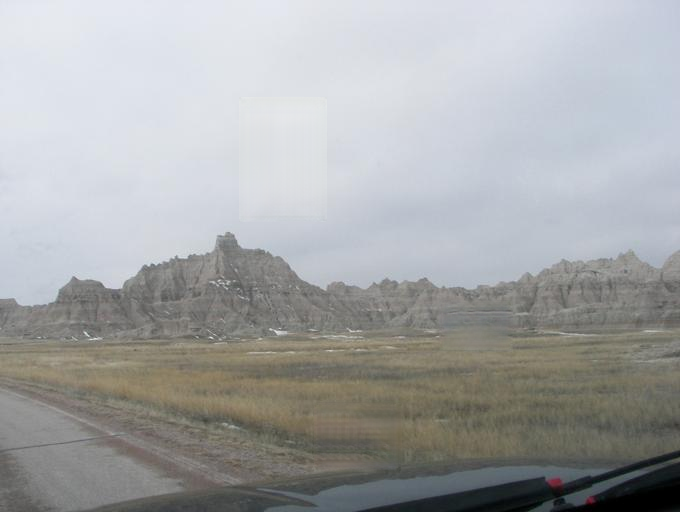
\includegraphics[width=.95\linewidth]{documentation/img/baseline/0185.png}
    \caption{Example n.11 -- Yu (baseline).}
    \label{img:ex_n.11_mask}
\end{figure}
\begin{figure}
    \centering
    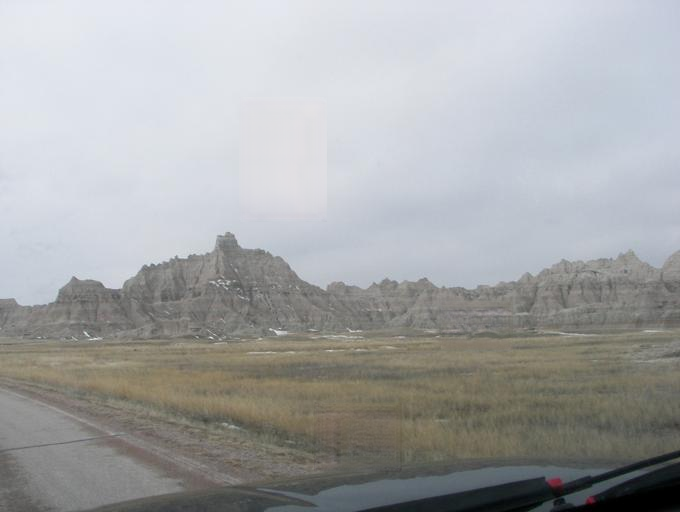
\includegraphics[width=.95\linewidth]{documentation/img/modified/0185.png}
    \caption{Example n.11 -- ours.}
    \label{img:ex_n.11_mask}
\end{figure}

\begin{figure}
    \centering
    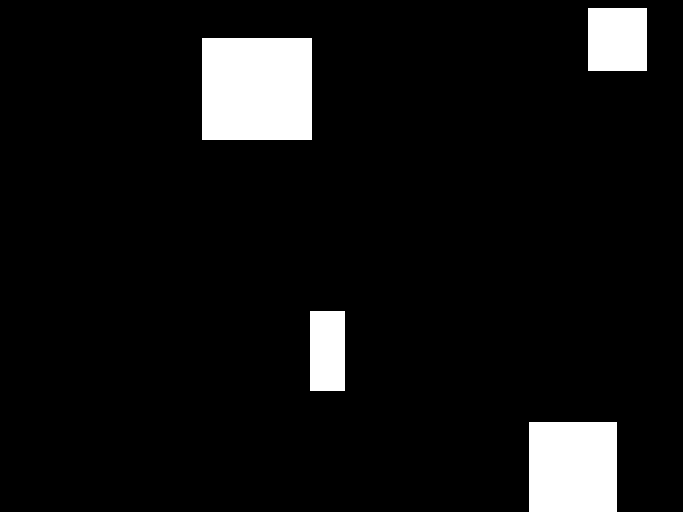
\includegraphics[width=.95\linewidth]{documentation/img/masks/0199_mask.png}
    \caption{Example n.12 -- mask.}
    \label{img:ex_n.12_mask}
\end{figure}
\begin{figure}
    \centering
    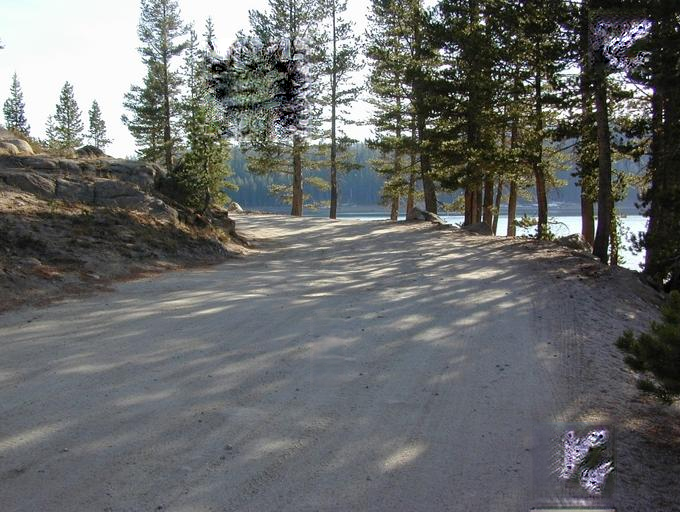
\includegraphics[width=.95\linewidth]{documentation/img/baseline/0199.png}
    \caption{Example n.12 -- Yu (baseline).}
    \label{img:ex_n.12_mask}
\end{figure}
\begin{figure}
    \centering
    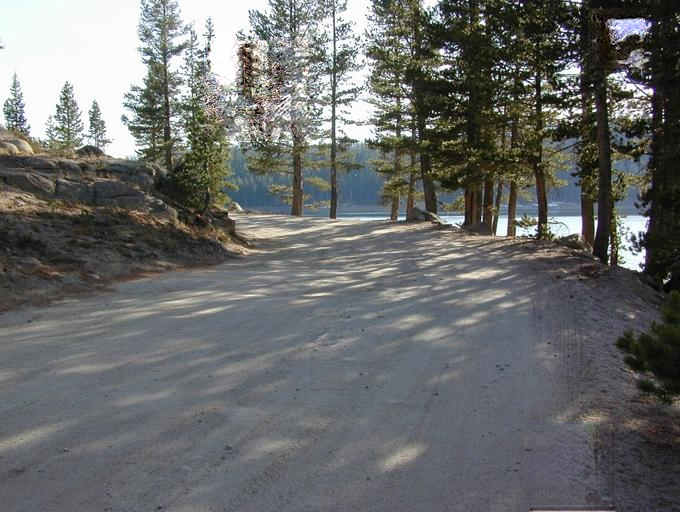
\includegraphics[width=.95\linewidth]{documentation/img/modified/0199.png}
    \caption{Example n.12 -- ours.}
    \label{img:ex_n.12_mask}
\end{figure}

\makeatletter
\def\@openbib@code{\addcontentsline{toc}{chapter}{Bibliography}}
\makeatother
\bibliographystyle{enplain}

\begin{flushleft}
\bibliography{bibliography}
\end{flushleft}

\end{document}
